\chapter{Testing and experimenting}


\section{Overall Approach to Testing and Experiments}
In the sense of this project testing was carried out for multiple purposes. From a software development point of view testing was carried out to ensure that the app performed as expected, where as from the research perceptive of this project testing was carried out to determine whether hybrid apps are feasible alternatives to native apps.

The acceptance and unit testing was carried out to test the actual functionality of the app and that the software performs as expected. The user testing and resource testing was more the experimental side to testing as it helped answer the research element to this project.

\section{Acceptance Testing}
It was important that all of the stories and features of the app worked properly as this would help with the user testing. Whilst there was no business or end user who specifically gave the project the requirements this stimulated. A table was derived which broke down all of the stories into multiple different features. These features were then tested, and a comment was left if the test did not pass.

\begin{center} 
 \begin{tabular}{||c c c c||}  
 \hline
 Story & Feature Name & Pass/Fail & Comment \\
 \hline\hline
 Registration and Login & Register User Details &  Fail &  \begin{tabular}{@{}c@{}} Users postcode \\ does not get\\ added properly \end{tabular} \\
 \hline
 Registration and Login & \begin{tabular}{@{}c@{}}Login with \\ previously created \\ account \end{tabular} & Pass &  Works as expected \\
 \hline
 Registration and Login & Logout & Fail & \begin{tabular}{@{}c@{}} System appears to \\ logout okay however \\ it loads previous \\ users feed. \end{tabular} \\
 \hline
 Profile Page & \begin{tabular}{@{}c@{}} Upload picture \\ from library \end{tabular}  &  Pass  & Works as expected  \\ 
 \hline
Profile Page & \begin{tabular}{@{}c@{}}Take picture \\using device's camera \\ and upload.\end{tabular} & Pass &  Works as expected  \\ 
\hline
Profile Page & Update bio & Pass & Works as expected \\
\hline 
Post System & User Posts & Pass &  \begin{tabular}{@{}c@{}} User posts get \\ added to feed table \\ as expected. \end{tabular} \\
\hline
Follow System & \begin{tabular}{@{}c@{}} User can follow \\ other users \end{tabular} & Pass &  \begin{tabular}{@{}c@{}} adds data to \\ the correct table \\ and shows as followed \\ on the app \end{tabular} \\
\hline
Follow system &  \begin{tabular}{@{}c@{}} User can unfollow \\ other users \end{tabular} & Pass &  \begin{tabular}{@{}c@{}} Can successfully unfollow other users \end{tabular} \\
\hline
 \begin{tabular}{@{}c@{}} Post System \\ and Follow System \end{tabular} &  \begin{tabular}{@{}c@{}} Correct posts \\ display on users \\ home page \end{tabular} & Pass & The correct posts display \\
 \hline
 Create Events System & Create a Venue & Pass &  \begin{tabular}{@{}c@{}} All necessary details \\ are stored in the \\ back end appropriately \end{tabular} \\
\hline
 Create Events System & Create Events Themselves & Pass & \begin{tabular}{@{}c@{}} Events are \\ properly created \\ and have a correct \\ link to the appropriate \\ venue id. \end{tabular} \\
 \hline
 Search &  \begin{tabular}{@{}c@{}} User can search \\ for nearby events \end{tabular} & Pass &  \begin{tabular}{@{}c@{}} Uses device's GPS \\ correctly and compares \\ with events location \end{tabular} \\
 \hline
  Search &  \begin{tabular}{@{}c@{}} User can search \\ for nearby music \\ lovers and artists \end{tabular} & Pass &  \begin{tabular}{@{}c@{}} Uses device's GPS \\ correctly and compares \\ with events location \end{tabular} \\
  \hline
   Search &  \begin{tabular}{@{}c@{}} User can search \\ for events \\ which are happening \\ soon \end{tabular} & Pass &  \begin{tabular}{@{}c@{}} Correctly sorts \\ events by dates  \end{tabular} \\
  \hline
\end{tabular}
\end{center}
 \captionof{table}{User Acceptance Testing Table}
\vspace{5mm}

It is clear from Table 4.1 that in terms of acceptance testing some of the code contained bugs for example the logout system was not working properly. Once all of the issues in Table 4.1 had been addressed another table; Table 4.2 was created, this goes through the tests which failed in Table 4.2 and evaluates whether they now pass.

\begin{center} 
 \begin{tabular}{||c c c c||}  
 \hline
 Story & Feature Name & Action Taken & Now Pass/Fail \\
 \hline\hline
 Registration and Login & Register User Details & \begin{tabular}{@{}c@{}} API amended \\ so that the \\ postcode variable \\ is now assigned \\ properly \end{tabular} & Pass \\
 \hline
 Registration and Login & Logout & \begin{tabular}{@{}c@{}} Now clears \\ cache on logout \end{tabular} & Pass \\
 \hline
 \end{tabular}
 \end{center}
 \captionof{table}{Corrections of failures from initial user acceptance testing}

\section{Unit tests}
It is important to unit test each of the main functions within the controllers to make sure that the user of the app wont encounter any weird behaviour. The Jasmine and Karma frameworks were used for unit testing the app \cite{testing}.

Figure 4.1 gives a small extract of the login unit test (the whole logintest.js file can be found in the appendix) which was wrote this unit test actually tests login controller. The unit tests work in such a way that the developer describes the function, followed by saying what the function should do and finally 

\begin{figure}[H]

\begin{verbatim}
describe('#doLogin', function() {
  it('Should Login using correct details', function() {
    expect(loginMock.doLogin).toHaveBeenCalledWith
    ('sea6@aber.ac.uk', 'b261la'); 
  });

  describe('when the login action is performed,', function() {
    it('if successful, should change state to home', function() {
      expect(stateMock.go).toHaveBeenCalledWith('app.home');
    });

    it('if unsuccessful, should show a popup', function() {
      expect(ionicPopupMock.alert).toHaveBeenCalled();
    });
  });
})
\end{verbatim}
\caption{Sample of unit test for login}
\end{figure}

Table X illustrates the different unit tests which were created (the tests can be viewed within the technical hand in.) and what functions were tested using these unit tests. Not every function was tested as some functions were very similar to functions in other controllers.

\begin{tabular} {||c c c c||}  
\hline
 Controller Name & Function Tested & What should happen & Name of Testing File\\
 \hline
 \hline 
 Login & doLogin & Login with details & logintest.js \\
 \hline
 Login & register &Move to registration screen & logintest.js \\
 \hline
 Register & doRegistration & Register with details & registertest.js \\
 \hline
 Register & returnToLogin & Change state to login & registertest.js \\
 \hline
 Home & postStatus & Post a status and popup should appear & hometest.js \\
 \hline
 \end{tabular}
  \captionof{table}{Table which shows different unit tests}


\section{User Interface testing}
For a mobile app user interface testing is very important. As the user interface is essentially how the user natvigates around the front end and how they submit data to the back end. Whilst there is no simple automatic way to test the UI on a ionic application, a table was derived which shows all of the different buttons and navigation options to ensure that the UI worked as expected.

\begin{center} 
 \begin{tabular}{||c c c c||}  
 \hline
 Location & Button/Navigation & Pass/Fail & Comment \\
 \hline
 Login Screen & Register Button & Pass & \begin{tabular}{@{}c@{}} Takes to registration \\ screen as expected. \end{tabular} \\
 \hline
 Login Screen & Login Button & Pass & \begin{tabular}{@{}c@{}} Logs the user \\ in if credentials are \\ correct if not it \\ displays an error message. \end{tabular} \\
 \hline
 Registration Screen & Return to Login Button & Pass & \begin{tabular}{@{}c@{}} App returns to \\ login screen on button \\ click. \end{tabular} \\
 \hline
 Registration Screen & Register Button & Pass & \begin{tabular}{@{}c@{}} Creates an account \\ if user has entered \\ correct information or \\ displays an error if \\ invalid info entered. \end{tabular} \\
 \hline
 \begin{tabular}{@{}c@{}} Menu (Shared across \\ multiple pages once \\ user is logged \\ in.) \end{tabular} & 'Home' link & Pass & \begin{tabular}{@{}c@{}} Take user to \\ the home page. \end{tabular} \\
 \hline
 \begin{tabular}{@{}c@{}} Menu (Shared across \\ multiple pages once \\ user is logged \\ in.) \end{tabular} & 'Artists' link & Pass & \begin{tabular}{@{}c@{}} Takes user to \\ artists page. \end{tabular} \\
 \hline
 \begin{tabular}{@{}c@{}} Menu (Shared across \\ multiple pages once \\ user is logged \\ in.) \end{tabular} & 'Events' link & Pass & \begin{tabular}{@{}c@{}} Takes user to \\ events page. \end{tabular} \\
 \hline
 \begin{tabular}{@{}c@{}} Menu (Shared across \\ multiple pages once \\ user is logged \\ in.) \end{tabular} & 'Music Lovers' link & Pass & \begin{tabular}{@{}c@{}} Takes user to \\ music lovers page. \end{tabular} \\
 \hline
 \begin{tabular}{@{}c@{}} Menu (Shared across \\ multiple pages once \\ user is logged \\ in.) \end{tabular} & 'My Profile' link & Pass & \begin{tabular}{@{}c@{}} Takes user to \\ my profile page. \end{tabular} \\
 \hline
 \begin{tabular}{@{}c@{}} Menu (Shared across \\ multiple pages once \\ user is logged \\ in.) \end{tabular} & 'Logout' link & Pass & \begin{tabular}{@{}c@{}} Logs user out \\ and returns them \\ to login page. \end{tabular} \\
 \hline
 \begin{tabular}{@{}c@{}} Menu (extras only \\ for venue owners.) \end{tabular}& 'Add a venue' link & Pass & \begin{tabular}{@{}c@{}} Takes venue owner \\ to add a \\ venue page. \end{tabular} \\
 \hline
 \begin{tabular}{@{}c@{}} Menu (extras only \\ for venue owners.) \end{tabular}& 'Make event' link & Pass & \begin{tabular}{@{}c@{}} Takes venue owner \\ to add an \\ event page. \end{tabular} \\
 \hline
Home Page & Submit post button & Pass & \begin{tabular}{@{}c@{}} Button posts the \\ data as expected.\end{tabular} \\
 \hline
 \hline
  \end{tabular}
   \end{center}
     \begin{center} 
 \begin{tabular}{||c c c c||} 
    \hline
 Location & Button/Navigation & Pass/Fail & Comment \\
 \hline
 Artists & \begin{tabular}{@{}c@{}} Sort by 'Recommended \\ Music Lovers' \end{tabular} & Pass & Displays correct results \\
 \hline

Artists & \begin{tabular}{@{}c@{}} Sort by 'Nearby \\ Music Lovers' \end{tabular} & Pass & Displays correct results \\
 \hline
Artists & \begin{tabular}{@{}c@{}} Sort by 'Newly \\ Joined Music Lovers' \end{tabular} & Pass & Displays correct results \\
Artists & \begin{tabular}{@{}c@{}} Click 'more info' \\ link on a \\ artist. \end{tabular} & Pass & \begin{tabular}{@{}c@{}} Correctly navigates to \\ the individual artists \\ page. \end{tabular} \\
 \hline
Artist Individual Page & \begin{tabular}{@{}c@{}} 'Follow' button \end{tabular} & Pass & Correctly follows artist. \\
 \hline
Artist Individual Page & \begin{tabular}{@{}c@{}} 'Un Follow' button \end{tabular} & Pass & Correctly unfollows artist. \\
  \hline
Events & \begin{tabular}{@{}c@{}} Sort by \\ 'Recommended Events' \\ selected and sort \\ button clicked.\end{tabular} & Pass & Correctly sorts the events \\
 \hline
 Events & \begin{tabular}{@{}c@{}} Sort by \\ 'Nearby Events' \\ selected and sort \\ button clicked.\end{tabular} & Pass & Correctly sorts the events \\
 \hline
 Events & \begin{tabular}{@{}c@{}} Sort by \\ 'Near Your Home' \\ selected and sort \\ button clicked.\end{tabular} & Pass & Correctly sorts the events \\
 \hline
 Events & \begin{tabular}{@{}c@{}} Sort by \\ 'Date of Events' \\ selected and sort \\ button clicked.\end{tabular} & Pass & Correctly sorts the events \\
 \hline 
 Events & \begin{tabular}{@{}c@{}}More info pressed \\ on event. \end{tabular} & Pass & \begin{tabular}{@{}c@{}} Correctly navigates \\ to the individual \\ event. \end{tabular} \\
 \hline
 Individual Event & \begin{tabular}{@{}c@{}}'Add event to favourites' \\ clicked on event. \end{tabular} & Pass & \begin{tabular}{@{}c@{}} Correctly adds event \\ to user favourites. \end{tabular} \\
 \hline 
Individual Event & \begin{tabular}{@{}c@{}}'Remove event from favourites' \\ clicked on event. \end{tabular} & Pass & \begin{tabular}{@{}c@{}} Correctly removes event \\ from favourites. \end{tabular} \\
 \hline
Add a venue & Register venue button pressed & Pass & \begin{tabular}{@{}c@{}} Creates venue on \\ button click or displays \\ error message if fields \\ are missing. \end{tabular} \\
\hline
Add an Event & Register event button pressed  & Pass & \begin{tabular}{@{}c@{}} Creates event on \\ button click or displays \\ error message if fields \\ are missing. \end{tabular} \\
\hline
\hline
 \end{tabular}
  \end{center}
 \begin{center}
 \begin{tabular}{||c c c c||}  
    \hline
     Location & Button/Navigation & Pass/Fail & Comment \\
     \hline \hline
General & User swipes screen left  & Pass & \begin{tabular}{@{}c@{}} Shows menu \\ as expected. \end{tabular} \\
\hline
General & \begin{tabular}{@{}c@{}} User swipes screen right \\ when menu open \end{tabular} & Pass & \begin{tabular}{@{}c@{}} Closes menu \\ as expected. \end{tabular} \\
\hline
\hline
 \end{tabular}
 \end{center}

\section{User testing}
In terms of user testing the actual questions which were discussed in the experimental methods section (see Appendix X), all of the questions were measure on a scale of 1 to 10 with 10 meaning that the user found the hybrid app fast and 1 meaning it was slow. table X shows the results.

\begin{center} 
 \begin{tabular}{||c c c c c c c||}  
 \hline
  \hline
 Participant & Q1 & Q2 & Q3 & Q4 & Q5 & Q6 \\
 \hline
 2 & 9 & 6 & 8 & 4 & 9 & 9 \\
 \hline
 3 & 10 & 9 & 9 & 4 & 8 & 4 \\
 \hline
 \hline
 \end{tabular}
 \end{center}

 Figure X gives a graphical representation of the results. 

 \section{Resource Usage}
 When considering if hybrid mobile application it is also important to consider how much of the devices resources the app is using. For comparison the resource usage of Facebook has also been listed.

 One of the main resources which was compared was the amount of CPU, as shown in Figure X when Facebook was looking for events it used 6\% where as when the hybrid app which was developed was also 6\%. It does need to be considered that Facebook is significantly larger than the hybrid app which was created consequently the hybrid app uses more CPU for less data than Facebook.

 Figure X shows 

\begin{figure}[H]
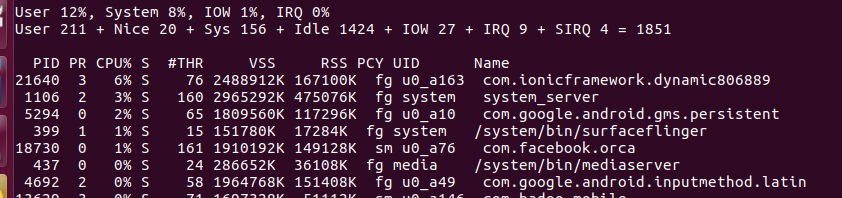
\includegraphics[scale=0.45]{images/ram2}
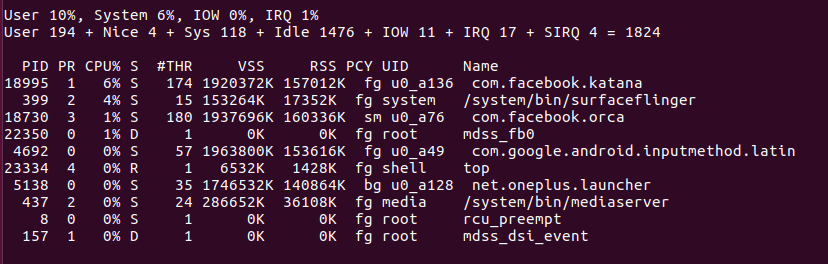
\includegraphics[scale=0.45]{images/ram3}
\caption{Images showing Facebook and Dynamic CPU.}
\end{figure}
